\chapter{Simulation Model Implementation}

\addcontentsline{toc}{chapter}{Simulation Model Implementation}

\section{Main Entities}

This chapter is going to describe the process of implementation, i.e. transition from a mathematical model to computer simulation. First of all we are going to create the basic elements that are essential to our model.

%\begin{figure}[!ht]
%  \centering
%  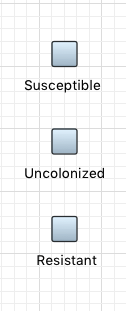
\includegraphics[height=0.5\textwidth]{img/screens/basic/basic4}
%  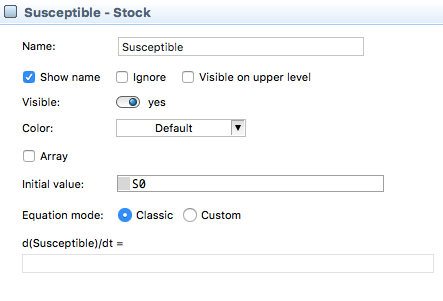
\includegraphics[height=0.5\textwidth]{img/screens/basic/basic3}
%  \caption{A picture of a gull.}
%\end{figure}

\begin{figure}[!ht]
    \centering
    \begin{subfigure}[b]{0.3\textwidth}
        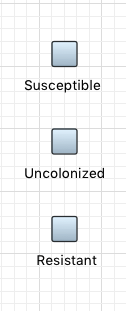
\includegraphics[width=0.5\textwidth]{img/screens/basic/basic4}
        \caption{The stocks of 3 observed groups}
    \end{subfigure}
    ~ %add desired spacing between images, e. g. ~, \quad, \qquad, \hfill etc.
      %(or a blank line to force the subfigure onto a new line)
    \begin{subfigure}[b]{0.6\textwidth}
        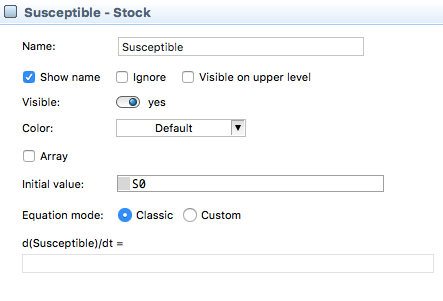
\includegraphics[width=\textwidth]{img/screens/basic/basic3}
        \caption{The properties of the Susceptible stock}
    \end{subfigure}
    \caption{Creation of the basic stock elements}
\end{figure}